% !TEX TS-program = pdflatex
% !TEX encoding = UTF-8 Unicode

% This is a simple template for a LaTeX document using the "article" class.
% See "book", "report", "letter" for other types of document.

\documentclass[11pt]{article} % use larger type; default would be 10pt

%\usepackage[utf8]{inputenc} % set input encoding (not needed with XeLaTeX)


%%% Examples of Article customizations
% These packages are optional, depending whether you want the features they provide.
% See the LaTeX Companion or other references for full information.

%%% PAGE DIMENSIONS
\usepackage{geometry} % to change the page dimensions
\geometry{a4paper} % or letterpaper (US) ocher a5paper or....
\geometry{margin=1in} % for example, change the margins to 2 inches all round
% \geometry{landscape} % set up the page for landscape
%   read geometry.pdf for detailed page layout information
\usepackage{graphicx} 
% \usepackage[parfill]{parskip} % Activate to begin paragraphs with an empty line rather than an indent

%%% PACKAGES
%\usepackage{booktabs} % for much better looking tables
\usepackage{array} % for better arrays (eg matrices) in maths
%\usepackage{paralist} % very flexible & customisable lists (eg. enumerate/itemize, etc.)
\usepackage{verbatim} % adds environment for commenting out blocks of text & for better verbatim
%\usepackage{subfig} % make it possible to include more than one captioned figure/table in a single float
% These packages are all incorporated in the memoir class to one degree or another...

%%% HEADERS & FOOTERS
\usepackage{fancyhdr} % This should be set AFTER setting up the page geometry
\pagestyle{fancy} % options: empty , plain , fancy
\renewcommand{\headrulewidth}{0pt} % customise the layout...
\lhead{}\chead{}\rhead{}
\lfoot{}\cfoot{\thepage}\rfoot{}

%%% SECTION TITLE APPEARANCE
%\usepackage{sectsty}
%\allsectionsfont{\sffamily\mdseries\upshape} % (See the fntguide.pdf for font help)
% (This matches ConTeXt defaults)

%%% ToC (table of contents) APPEARANCE
%\usepackage[nottoc,notlof,notlot]{tocbibind} % Put the bibliography in the ToC
%\usepackage[titles,subfigure]{tocloft} % Alter the style of the Table of Contents
%\renewcommand{\cftsecfont}{\rmfamily\mdseries\upshape}
%\renewcommand{\cftsecpagefont}{\rmfamily\mdseries\upshape} % No bold!

%\usepackage[T1]{fontenc}
\usepackage[latin9]{inputenc}
%\usepackage[active]{srcltx}
\usepackage{setspace}
\usepackage{lscape}
\doublespacing
\usepackage[english]{babel}
\bibliographystyle{naturemag}



\begin{document}

\title{Approaches for Enabling Deep, Large Scale Metagenome Assembly}
\author{ACH, JJ, ST, JMT, CTB}
\maketitle

\section{Introduction}  
Complex microbial communities operate at the heart of many crucial environmental, ecological, and biomedical processes, providing critical ecosystem functionality that underpins much of biology (\cite{Arumugam:2011p735,Hess:2011p686,Iverson:2012p1281,Mackelprang:2011p1087,Qin:2010p189,Tringe:2005p174,Venter:2004p170}).  These systems are difficult to study in situ, and consequently, we lack a fundamental understanding of their diversity and function, much less how they self-assemble, maintain themselves, and evolve through time.  Advances in DNA sequencing technologies now provide unprecedented access to these communities in the form of millions to billions of short-read sequences of community DNA  \cite{Hess:2011p686,Mackelprang:2011p1087,Qin:2010p189}.   Even more sequencing is needed to detect the rare species in environmental samples, e.g., up to 50 Tbp for an individual gram of soil \cite{Gans:2005p1365}.   Both the read lengths and volume of sequencing data pose new challenges to traditional analysis approaches of sequencing data.  Short read lengths and their associated sequencing errors and biases contain little biological signal and are noisy, limiting direct annotation approaches against known reference genomes.  Further complicating analysis is that the majority of genes sequenced from metagenomes are not similar to known genes \cite{Arumugam:2011p735,Qin:2010p189}.  

\emph{De novo} assembly of raw sequencing data offers several advantages for studying  sequencing datasets.  It both reduces the presence  of sequencing errors and the total number of sequences for analysis by identifying consensus sequences from overlapping reads.  These resulting assembled contigs are longer than sequencing reads and provide gene order.  Importantly, \emph{de novo} assembly does not rely on the existence of reference genomes, thus allowing for the discovery of novel elements.   The main challenge for metagenomic applications of \emph{do novo} assembly is that current assembly tools do not scale to the volumes of metagenomic datasets being generated: metagenomes assembled from rumen, human gut, and permafrost soil sequencing could only be assembled after sample preprocessing to discard low abundance sequences \cite{Hess:2011p686,Mackelprang:2011p1087,Qin:2010p189}.  Traditional assemblers have been designed for the assembly of single genomes whose abundance distribution and diversity content are significantly different from the mixed populations of metagenomes, and although many new metagenome-specific assemblers have been developed to address characteristics of mixed population assembly, these are limited in capacity of sample diversity and volume.    

Here, we present a novel set of approaches which enable large-scale metagenomic de novo assembly.  The first approach reduces the dataset size by discarding reads from high-coverage regions.  Subsequently, reads are separated based on asembly graph connectivity, resulting in easily assembled partitions.   We evaluate these approaches using the assembly of a human gut mock community dataset and find that our methods result in assemblies nearly identical to assemblies from the unprocessed dataset.  Next, we apply our approaches towards the assembly of two previously intractable soil metagenomes, one from Iowa agricultural soil under continuous cultivation, and one from native Iowa prairie.  We compare the predicted functional capacities and phylogenetic content of the assemblies and conclude that despite significant phylogenetic differences, the functions encoded in both soil data sets are similar.  We also show that there is virtually no strain-level heterogeneity dectable within these samples.

\section{Results}

\subsection{Assembly of the HMP mock metagenome}

\subsubsection{Evaluation of data reduction through digital normalization and high abundance filtering}

The recovery of reference genomes from de novo metagenomic assembly was evaluated, comparing unfiltered traditional assembly to the the described filtered assembly (See Methods and Supp Info). Initially, the abundance of genomes within the mock dataset was estimated based on the reference genome coverage of sequencing reads in the unfiltered dataset.  Coverage (excluding genomes with less than 3-fold coverage) ranged from 6-fold to 2,000-fold coverages (Supp. Table ~\ref{referencestats} and Supp Fig. ~\ref{coverage1} and ~\ref{coverage2}).  Overall, the unfiltered dataset reads covered a total of 93\% of the reference genomes.  During filtering, a total of 5.9 million reads (40\% of total reads) contributing to dataset redundancy and sequencing errors and biases (Supp. Info digital normalization and high abundance filtering) were removed.  The remaining reads covered a total of 91\% of the available reference genomes (Table ~\ref{data-summary} and Supp. Figures coverage1 and coverage2).   

Additionally, the recovery of reference genomes by the contigs assembled from the original and filtered datasets were compared, resulting in recoveries of 43\% and 44\% of references (Velvet assembler), respectively.  The assembly of the original dataset contained 29,063 contigs and 38 million bp compared to the filtered assembly containing 30,082 contigs and 35 million bp (Table ~\ref{assembly-summary}).  Comparable recoveries of references between original and filtered datasets were also obtained for other assemblers (SOAPdenovo and Meta-IDBA).   Overall, the unfiltered and filtered assemblies were were similar, sharing ~95\% genomic content.   For the highest abundance genomes (e.g., ref\textbar{}NC\_005008.1, ref\textbar{}NC\_005007.1, and ref\textbar{}NC\_005003.1), the unfiltered assembly recovered significantly more of the original genomes; however, for the large majority of genomes the filtered assembly recovered similar (and sometimes greater) amounts of the reference genomes Supp Fig X and X).  The distribution of contig lengths in unfiltered and filtered assemblies were also comparable (Supp Figure X).

The abundance of assembled contigs and reference genomes could be recovered using the coverage of sequencing reads (Supp Fig ~\ref{diginormreference}).  In general, a minimum depth of sequencing was observed when contigs were assembled. Above a sequencing coverage of five, the majority of reads which could be mapped to reference genomes were likely to be included in an assembled contig (Supp Fig. ~\ref{coveragehmp}).  Below this threshold, reads could be mapped to reference genomes but were less likely to be associated with assembled contigs.  Using the reference genomes, assembly-based abundance estimations of references could be evaluated, and the estimations based on unfiltered and filtered assemblies compared.  The abundance estimations from the filtered assembly were significantly closer to predicted abundances from reference genomes (p-value of 0.032, see Supp Info).  

\subsubsection{Evaluation of partitioning reads based on connectivity}
To divide the the remaining dataset, the filtered dataset was partitioned based on connectivity within a de Bruijn graph representation (previously described in Pell et al. and Howe et al.), and each partition was assembled independently.  The resulting assemblies of filtered, unpartitioned and filtered, partitioned datasets were compared and found to be greater than 99\% identical.  For the mock dataset, a total of 85,818 disconnected partitions (a total of 9 million reads) containing a minimum of five reads were identified (Fig. ~\ref{ecolimap}).  Among these, only 2,359 partitions contained reads originating from more than one genome, indicating that partitioning properly separated reads from distinct species.
%With the exception of one partition containing reads from 36 reference genomes, all other partitions contained reads from less than a total of nine genomes.  
In general, reference genomes with high sequencing coverage were associated with fewer partitions (Supp Table ~\ref{referencestats}), a total of 112 partitions contained reads from high abundance reference genomes (coverage above 25) compared to 2,771 partitions associated with low abundance genomes (coverage below 25).   %As expected, reads aligning to similar regions of a reference genome were found to be associated with the the same partition (SI Fig. ~\ref{partitionreference}).

To further evaluate the effects of partitioning, spiked reads from \emph{E. coli} genomes were introduced into the mock community dataset. A single spiked genome (\emph{E. coli} strain E24377A, NC\_009801.1 with 2\% error)) was added to the mock community dataset and processed identically to the unfiltered mock dataset.  Similar amounts of data reduction after digital normalization and partitioning (Table ~\ref{data-summary}) were observed.  Among the 81,154 partitioned sets of reads, we identified only 2,580 partitions containing reads from multiple genomes.  A total of 424 partitions contained reads from the spiked \emph{E. coli} genome (201 partitions contained \emph{only} spiked reads) and when assembled aligned with 99.5\% of \emph{E. coli} strain E24377A genome (4,957,067 of 4,979,619 bp) (Fig. ~\ref{ecolimap}).  Next, the same analysis was performed on the mock dataset after introducing five closely-related \emph{E. coli} strains into the mock community dataset.  Partitioning this ``mix-spiked" mock community dataset resulted in 81,425 partitions, of which 1,154 partitions contained reads associated with multiple genomes.  Among the partitions which contained reads associated with a single genome, 658 partitions contained reads originating from one of the spiked \emph{E. coli} strains.  In partitions containing greater than one genome, 224 partitions contained reads from a spiked \emph{E. coli} strain and one other reference genome (either another spiked strain or from the mock community dataset) (Fig. ~\ref{ecolimap2}).  The partitions containing reads originating from the spiked \emph{E. coli} strains were identified and assembled independently.  Among the resulting 6,076 contigs, all but three contigs could be identified as originating from a spiked \emph{E. coli} genome (e.g., top blast hit).  The remaining three contigs were greater than 99\% similar to HMP mock reference genomes (NC\_000915.1, NC\_003112.2, and NC\_009614.1).  The contigs associated with \emph{E. coli} were aligned against the spiked reference genomes, recovering greater than 98\% of each of the five genomes.  Many of these contigs were associated with reads originating from multiple genomes (Supp Fig. ~\ref{fractionassembled}), 3,075 contigs (51\%) could be aligned to reads which originated from more than one spiked genome.  This result is comparable to the fraction of contigs which are associated with multiple genomes when the unfiltered dataset is assembled, where in 4,702 contigs associated with ``spiked reads", 66\% contained reads originating from more than one spiked genome.

\subsection{Characteristics of soil metagenomes}

We next applied these approaches to the de novo assembly of two soil metagenomes.  Previously, the assembly of the Iowa corn and prairie datasets (containing 1.8 billion and 3.3 billion reads, respectively) were impossible to assemble with readily available memory, e.g., 500 GB.   A 75 million reads subset of the Iowa corn dataset alone required 110 GB of memory (Supp Fig. ~\ref{memory}).  Applying the same filtering approaches as described above, the Iowa corn and prairie datasets were reduced to 1.4 billion and 2.2 billion reads, respectively, and after partitioning, a total of 1.0 billion and 1.7 billion reads remained, respectively.  Notably, the Iowa corn and prairie were sampled at significantly lower sequencing coverages than the mock community.  %i.e., the mock dataset had only 33\% of its k-mers (k=20) present less than ten-times in the dataset, while the Iowa corn and prairie datasets contained 53\% and 43\%, respectively, of all k-mers with less than ten-fold coverage.  
The large majority of k-mers in the soil metagenomes are relatively low-abundance (Fig. ~\ref{diginormcoverage}), and consequently, digital normalization did not remove as many reads in the soil metagenomes.

\subsubsection{Assembly of soil metagenomes}

Based on the mock community dataset, we estimated that above a sequencing depth of six, the large majority of sequences could be assembled (Supp. Fig. ~\ref{coveragehmp}).  Given the greater diversity expected in the soil metagenomes, we normalized these datasets to a coverage threshold of 20.  After partitioning the filtered datasets, a total 31,537,798 and 55,993,006 partitions (containing greater than five reads) in the corn and prairie datasets, respectively, were identified.  For practical assembly, partitions were grouped together such that groups contained partitions with similar numbers of reads and no group contained larger than 10 million reads.  Once partitioned, each group of reads could be assembled in less than 14 GB and 4 hours, enabling evaluation of multiple assemblers and various assembly parameters. 

The final assembly of the corn and prairie soil metagenomes resulted in a total of 1.9 million and 3.1 million contigs (Velvet), respectively, and a total assembly length of 912 million bp and 1.5 billion bp, respectively.  To estimate abundance of assembled contigs and evaluate incorporation of reads, all quality-trimmed reads were aligned to assembled contigs (greater than 300 bp).  Overall, for the Iowa corn assembly, 8\% of single reads and 10\% of paired end reads mapped to the assembly.  Among the paired end reads, less than 0.5\% aligned disconcordantly.  Similar results were found for the Iowa prairie assembly where only 0.6\% paired ends aligned disconcordantly and slightly increased numbers of reads mapped with 10\% of single reads and 11\% paired end reads (Table ~\ref{read-map}).  Based on these mappings, the read coverage of assembled contigs within the soil metagenomes were estimated (Fig. ~\ref{soilassemblycoverage}).  Overall, there is a positively skewed distribution of coverage of all contigs from both soil metagenomes, biased towards a coverage of less than ten-fold.  The Iowa corn and prairie assemblies contained 48\% and 31\% of total contigs with a median basepair coverage less than 10.  

Among contigs, the presence of polymorphisms was examined by identifying the amount of consensus obtained by reads mapped (Supp. Info methods).  For both the Iowa corn and prairie metagenomes, nearly all assembled sequences (greater than 99.9\%) contained base calls which were supported by 95\% consensus from mapped reads over 90\% over its length (Supp. Fig Polymorphisms corn and prairie).  

%For the filtered datasets, the time and memory requirements for de novo assembly were significantly reduced.  The filtering took less than 4 hours, but the time and memory for assembly (Velvet) was reduced from 12 GB and 4 hours for the unfiltered dataset to 3 GB and less than 1 hour for the filtered datasets.   


\subsubsection{Content of soil metagenome assembly}

%The number of genomes represented in the Iowa corn and prairie assemblies was estimated through the identification of single copy recA and rplB genes within each metagenome.   We estimate the abundance of recA and rplB to be 3,329 and 3,209, respectively, in the Iowa corn and 3,541 and 2,018 in the Iowa prairie.  (I think we should remove this part out - or push the whole discussion in supplementary).

Assembled contigs with their respective bp-coverage (with a median bp coverage greater than 1) were annotated through the MG-RAST pipeline resulting in 2,089,779 and  3,460,496 predicted protein coding regions in the corn and prairie metagenomes, respectively.  The large majority of these regions did not share similarity with any gene in the M5NR database, 61.8\% in corn and 70.0\% in prairie.  In total, 613,213 and 777,454 protein coding regions were assigned to functional categories.  The functional profile of these annotated features against SEED subsystems were compared (Fig. ~\ref{subsystem}).  For both the corn and prairie metagenomes, the most abundant functions were associated with the carbohydrate (e.g., central carbohydrate metabolism and sugar utilization), amino acids (e.g., biosynthesis and degradation), and protein metabolism (e.g., biosynthesis, processing, and modification) subsystems.  The subsystem profile of both metagenomes were very similar while the taxonomic profile of the metagenomes based on the originating taxonomy (phyla) were different (Fig. ~\ref{phyla}, Supp Methods).  Within both metagenomes, Proteobacteria were the most abundant taxa.  However, in the Iowa corn, Actinobacteria followed by Bacterioidetes and Firmucutes were the next most abundant while in the Iowa prairie, Acidobacteria were the second most abundant phyla, followed by Bacterioidetes  and Actinobacteria.  The Iowa prairie also had nearly double the fraction of Verruomicrobia compared to the Iowa corn.  


\section{Discussion}

\subsection{Filtering approaches effectively reduce datasets} 

The diversity and sequencing depth represented by the mock community is extremely low compared to that of most environmental metagenomes; however, it represents a simplified, unevenly sampled model for a metagenomic dataset which enables the evaluation of analyses through the availability of source genomes.  For this dataset, the filtering approaches described above were effective at reducing the dataset size without significant loss of assembly.  This strategic filtering takes advantage of the observed coverage "sweet spot" at which point sufficient sequences are present for assembly and beyond which further sequencing is not productive (and increases the number of sources of errors) (Supp Fig X).    The normalization of sequences also results in a more even distribution of coverage (Fig. ~\ref{diginormcoverage}), minimizing assembly problems caused by highly variable coverage.  Additional reduction of the dataset was achieved by the removal of high abundance sequences, previously correlated as Illumina sequencing artifacts (Howe et al).  

The specific effects of filtering varied depending on differences of reference genomes.  Sequencing coverage and conserved regions among references had an impact on filtered assembly recovery.  The filtered assemblies of the three plasmids of the \emph{Staphylococcus} epidermidis genome (NC\_005008.1, NC\_005007.1, and NC\_005003.1) were highly abundant (Supp Tab X) and shared several conserved regions (~90\% identity over ~290 bp).  During normalization, repetitive elements in these genomes would appear as high coverage elements and be removed, evidenced by a large difference in the number of reads associated with NC\_005008.1 in the unfiltered and filtered datasets (Supp Fig X). Consequently, the unfiltered dataset contained more reads spanning these repetitive regions.  This most likely enabled assembler heuristics to extend the assembly of these sequences and resulted in the observed increased recovery of these genomes in the unfiltered assemblies. This result, though rare among the mock reference genomes, identifies a shortcoming of our approach, and indeed for most short-read assembly approaches, related to repetitive regions and/or polymorphisms.  For the soil metagenomes, our data reduction may cause some information loss which may have been useful for assembly, but the benefit of being able to assemble previously intractable datasets is obvious.  Evaluation with the mock community dataset suggests that this information loss is minimal overall and that our approaches result in a comparable assembly whose abundance estimations are similar, if not improved.     

\subsection{Partitioning effectively separates genomes for assembly}

A broad range of diversity must be represented in metagenomic assembly graphs.   These graphs contain continuous paths of short, overlapping sequences which are used to determine read overlaps.  Two or more genomes which are thoroughly sequenced would be expected to be connected in a single assembly graph by conserved elements such as those within 16S rRNA genes.  For most metagenomes, however, the majority of constituent genomes are undersampled resulting in only fragments of connectivity.  Thus, these assembly graphs are expected to contain multiple, separate connected sets of reads or subgraphs representing sequences from different genomes or genomic fragments.  Our partitioning approach targets these subgraphs to divide large metagenomes into subsets which reflect the biological characteristics of the originating dataset.  

To enable partitioning of metagenomic datasets, sequencing biases which cause artificial connectivity within metagenomic assembly graphs were removed (high abundance sequence filtering) (Howe).  As discussed above, tthe removal of these sequences (combined with normalization) did not significantly alter the recovery of reference genomes through de novo assembly and importantly, it enabled the division of the mock community dataset into thousands of disconnected partitions.  The resulting assemblies of unpartitioned and partitioned datasets were nearly identical.  The large majority of these partitions  contained reads from a single reference genome, supporting our previous hypothesis that most connected subgraphs contain distinct genomes.  As expected, high coverage, well-sampled genomes were found to contain fewer partitions (highly connected assembly graph), and low coverage, under-sampled genomes contained more partitions (fragmented assembly graph).  

To further examine the recovery of sequences through partitioning, one or more \emph{E. coli} strains were computationally spiked into the mock community dataset.  For a spike of a single \emph{E. coli} strain, the fraction of partitions containing \emph{E. Coli} associated reads could be reassembled to recover 99\% of the original genome (Fig. ~\ref{ecolimap}).  When five closely related strains were spiked into the mock dataset, we could recover the large majority of the genomic content of these strains but largely in chimeric contigs (Supp Fig. ~\ref{fractionassembled}).  This result is not unexpected nor unique to our approach as assemblies of the unfiltered dataset resulted in a slightly higher fraction of assembled contigs associated with multiple references.  Overall, closely related sequences which result from either repetitive or inter-strain polymorphisms are a challenge to assemblers, and our approaches are not specifically designed to target such regions.  However, the partitions resulting from our approach (without digital normalization) could provide a subset of sequences which could be targeted for more sensitive assembly approaches for such regions (i.e. overlap-layout-consensus approaches or abundance binning approaches (cite Itai)).  

A valuable result of our partitioning approach is that it effectively subdivides our datasets into sets of reads which can be assembled in parallel, and consequently, with less computational resources.  For the mock community dataset, this gain was small, reducing unfiltered assembly at 12 GB and 4 hours to less than 2 GB and 1 hour.  However, for the soil metagenomes, previously impossible assemblies could be completed in less than a day and in under 14 GB of memory enabling the usage of multiple assembly parameters (e.g., k-length) and multiple assemblers (Velvet, Soapdenovo, and Meta-idba).

\subsection{Soil assembly}
The final assemblies of the corn and prairie soil metagenomes resulted in a total of 1.9 million and 3.1 million contigs, respectively, and a total assembly length of 912 million bp and 1.5 billion bp, respectively (equivalent to ? genomes).  Without references, these assemblies were evaluated based on paired-end concordance.  Overall, there is a positively skewed distribution of coverage of all contigs from both soil metagenomes, biased towards a coverage of less than ten-fold, indicative of the low sequencing overage of these metagenomes.  

%The Iowa corn and prairie assemblies contained 48\% and 31\% of total contigs with a median basepair coverage less than 10.  The presence of polymorphisms within assembled contigs was estimated based on the consensus sequences of reads mapped to each contig (see Supp. Info methods).  For both the Iowa corn and prairie metagenomes, nearly all assembled sequences (greater than 99.9\% of all contigs) contained base calls which were supported by 95\% consensus from mapped reads over 90\% over its length (Supp. Fig Polymorphisms corn and prairie).  

This study represents the largest soil metagenomic sequencing effort to date, and these assembly results demonstrate the enormous amount of diversity within the soil.  Even with this level of sequencing, hundred of thousands of functions were identified for each metagenome.  More than half of the assembled contigs are not similar to anything in known databases suggesting that de novo assembly of novel sequences holds great benefit for soil metagenomics.  Interestingly, among the protein coding sequences which were annotated, comparisons of the two soil datasets suggests that the functional profiles are more similar to one another than the complementing phylogenetic profiles.  This result supports previous hypotheses that despite large diversity with two different soil systems, the microbial community provides similar function (cite Kostas?, etc.).  

\section{Conclusion}
The key strategies presented here have focused firstly on systematically reducing metagenomic data by removing errors and sequence redundancy and secondly on the division of the remaining dataset informed by its biological connectivity.  Both of these approaches required understanding the underlying sequencing datasets requiring assembly, specifically the key differences in metagenomes and more traditional genome assembly approaches (e.g., variable coverage and diversity).   As the application of metagenomic sequencing for environmental studies grows in both volume and breadth, it is critical to re-evaluate traditional approaches which have developed from the genomic era.  Beyond assembly, approaches for quality control, estimating diversity, and statistical determination of signal from noise are all areas which need further development for metagenomics.  The methods described above allow for easy re-analysis of the metagenomes by providing datasets of a tractable size; thus, novel developments in assembly approaches (and other analysis such as binning or even annotation) can easily be evaluated.  The two metagenomic soil assemblies above provide a glimpse into the opportunities that metagenomic sequencing will provide, especially the high fraction of unknown proteins identified.  This technology is still in its infancy.  Thoughtful analytical approaches, like scalable de novo metagenomic assembly, combined with well-chosen experimental design and iterative discovery-driven research will accelerate the impact of metagenomic studies for scientific advances which will help society.

\subsection{Assembly Pipeline}
The entire assembly pipeline for the mock community is described in detail in an iPython notebook available for download at XXX accompanied by a web-based tutorial.  Soil assembly was performed with the same pipeline and parameter changes are described in Supp Info.

\bibliography{assembly-paper}

\section{Tables}

\begin{table}[ht]
\caption{The total number of reads in unfiltered, filtered (normalized and high abundance (HA) k-mer removal), and partitioned datasets and the computational resources required (memory and time).}
\begin{tabular}{l c c c c c}
& Unfiltered & Filtered & Partitioned & Filtering & Partitioning \\
& reads & reads & reads & GB / h & GB / h   \\
\hline
HMP Mock & 14,494,884 & 8,656,536 & 8,560,124 & 4 / $<$2 & 4 / $<$2 \\
HMP Mock Spike & 14,992,845 & 8,189,928 & 8,094,475 & 4 / $<$2 & 4 / $<$2 \\
HMP Mock Multispike & 17,010,607 & 9,037,142 & 8,930,840 & 4 / $<$2 & 4 / $<$2 \\
Iowa Corn & 1,810,630,781 & 1,406,361,241 & 1,040,396,940 & 188 / 83 & 234 / 120 \\
Iowa Prairie & 3,303,375,485 & 2,241,951,533 & 1,696,187,797 & 258 / 178 & 287 / 310 \\
\hline
\end{tabular}
\label{data-summary}
\end{table}

\begin{table}[ht]
\caption{Assembly summary statistics (total contigs, total million bp assembly length, maximum contig size bp) of unfiltered (UF) and filtered (F) or filtered/partitioned (FP) datasets with Velvet (V) assembler.  Assembly for UF and FP datasets also shown for MetaIDBA (M) and SOAPdenovo(S) assemblers.  Iowa corn and prairie metagenomes could not be completed on unfiltered datasets.}
\begin{tabular}{l c c c c}
& UF & F & FP & Assembler \\
\hline
HMP Mock & 29,063 / 38 / 146,795 & 30,082 / 35 / 90,497 & 30,115 / 35 / 90,497 & V \\
HMP Mock & 24,300 / 36  / 86,445 & - & 27,475 / 36 / 96,041 & M \\
HMP Mock & 36,689 / 37 / 32,736 & - & 29,295 / 37 / 58,598 & S \\
Iowa corn & N/A & N/A & 1,862,962 / 912/ 20,234 & V \\
Iowa corn & N/A & N/A & 1,334,841 / 623 / 15,013 & M \\
Iowa corn & N/A & N/A & 1,542,436 / 675 / 15,075 & S \\
Iowa prairie & N/A & N/A & 3,120,263 / 1,510 / 9,397 & V \\
Iowa prairie & N/A & N/A & 2,102,163 / 998 / 7,206 & M \\
Iowa prairie & N/A & N/A & 2,599,767 / 1,145 / 5,423 & S \\
\end{tabular}
\label{assembly-summary}
\end{table}

\begin{table}[ht]
\caption{Assembly comparisons of unfiltered (UF) and filtered (F) or filtered/partitioned (FP) HMP mock datasets using different assemblers (Velvet (V), MetaIDBA (M) and SOAPdenovo (S)).  Assembly content similarity is based on the fraction of alignment of assemblies and similarly, the coverage of reference genomes is based on the alignment of assembled contigs to reference genomes (RG).}
\begin{tabular}{l c c c}
Assembly Comparison & Percent Similarity & RG Coverage & Assembler \\
\hline
UF vs. F & 95\% & 43.3\% / 44.5\% & V \\
UF vs. FP & 95\% & 43.3\% / 44.4\% & V\\
UF vs. FP & 93\% & 46.5\% / 45.4\% & M\\ 
UF vs. FP & 98\% &  46.2\% / 46.4\% & S\\
\end{tabular}
\label{assembly-compare}
\end{table}

\begin{table}[ht]
\caption{Fraction of single-end (SE) and paired-end (PE) reads mapped to Iowa corn and prairie Velvet assemblies.}
\begin{tabular}{l c c}
 & Iowa Corn Assembly & Iowa Prairie Assemby \\
 \hline
Total Unfiltered Reads	& 1,810,630,781	& 3,303,375,485\\
Total Unfiltered SE Reads &	141,517,075 &	358,817,057\\
SE aligned 1 time	& 11,368,837	& 32,539,726\\
SE aligned $>$ 1 time	& 562,637	& 1,437,284\\
\% SE Aligned & 	8.43\% &	9.47\% \\
Total Unfiltered PE Reads & 	834,556,853	& 1,472,279,214\\
PE aligned 1 time	& 54,731,320	& 110,353,902\\
PE aligned $>$ 1 time	&1,993,902	 & 3,133,710\\
\% PE Aligned Disconcordantly	 & 0.47\% &	 0.63\%\\
\% PE Aligned	& 9.68\%	& 11.20\%\\
\end{tabular}
\label{read-map}
\end{table}




\pagebreak
\section{Figures}

\begin{figure}[ht]
\center{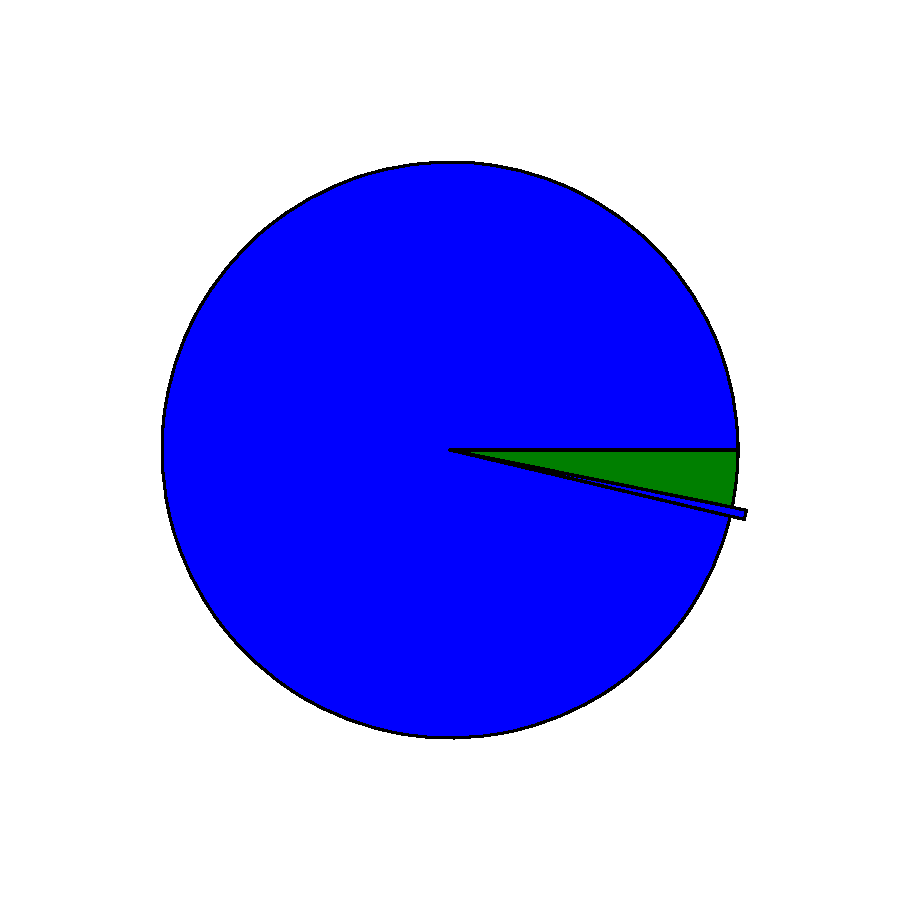
\includegraphics[width=\textwidth,height=\textheight,keepaspectratio]{./figures/singleecoli-pie.pdf}}
\caption{The fraction of partitions in spiked HMP dataset (single \emph{E. Coli}) which contain single genomes (blue) and multiple genomes (green).  The exploded pie chart section indicates partitions which contain spiked \emph{E. coli} reads which were subsequently assembled independently.}
\label{ecolimap}
\end{figure}

\begin{figure}[ht]
\center{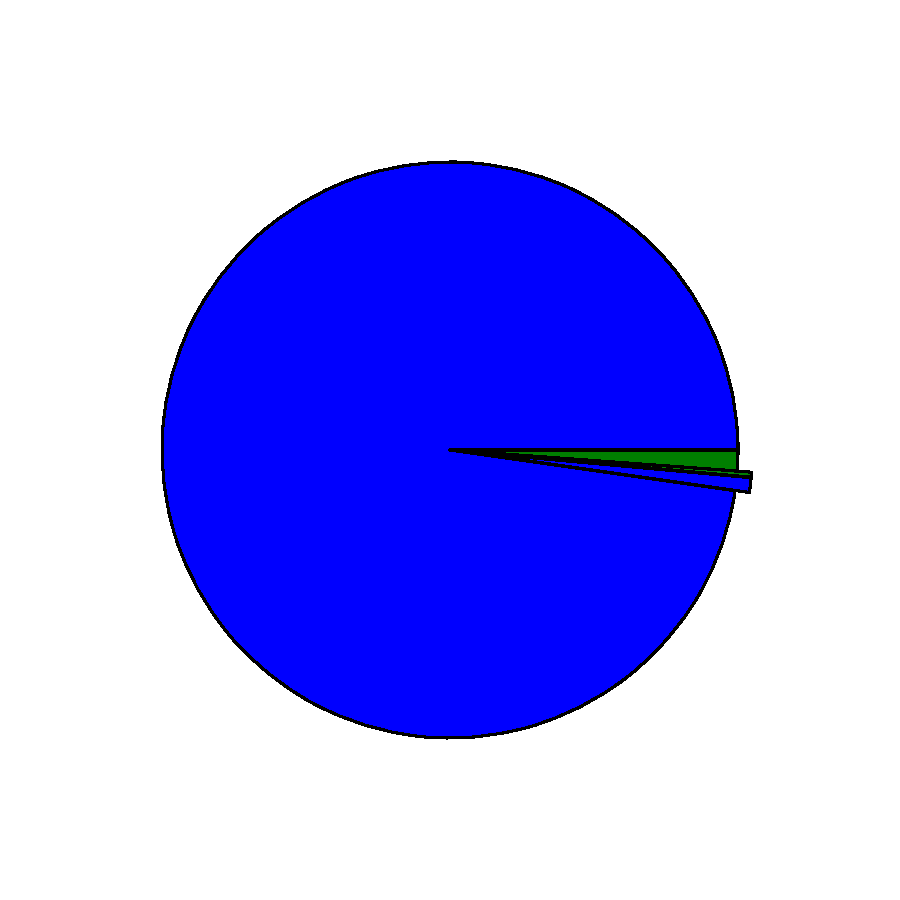
\includegraphics[width=\textwidth,height=\textheight,keepaspectratio]{./figures/multipleecoli-pie.pdf}}
\caption{The fraction of partitions in spiked HMP dataset (five \emph{E. Colis}) which contain single genomes (blue) and multiple genomes (green).  The exploded pie chart section indicates partitions which contain spiked \emph{E. coli} reads which were subsequently assembled independently. }
\label{ecolimap2}
\end{figure}


\begin{figure}[ht]
\center{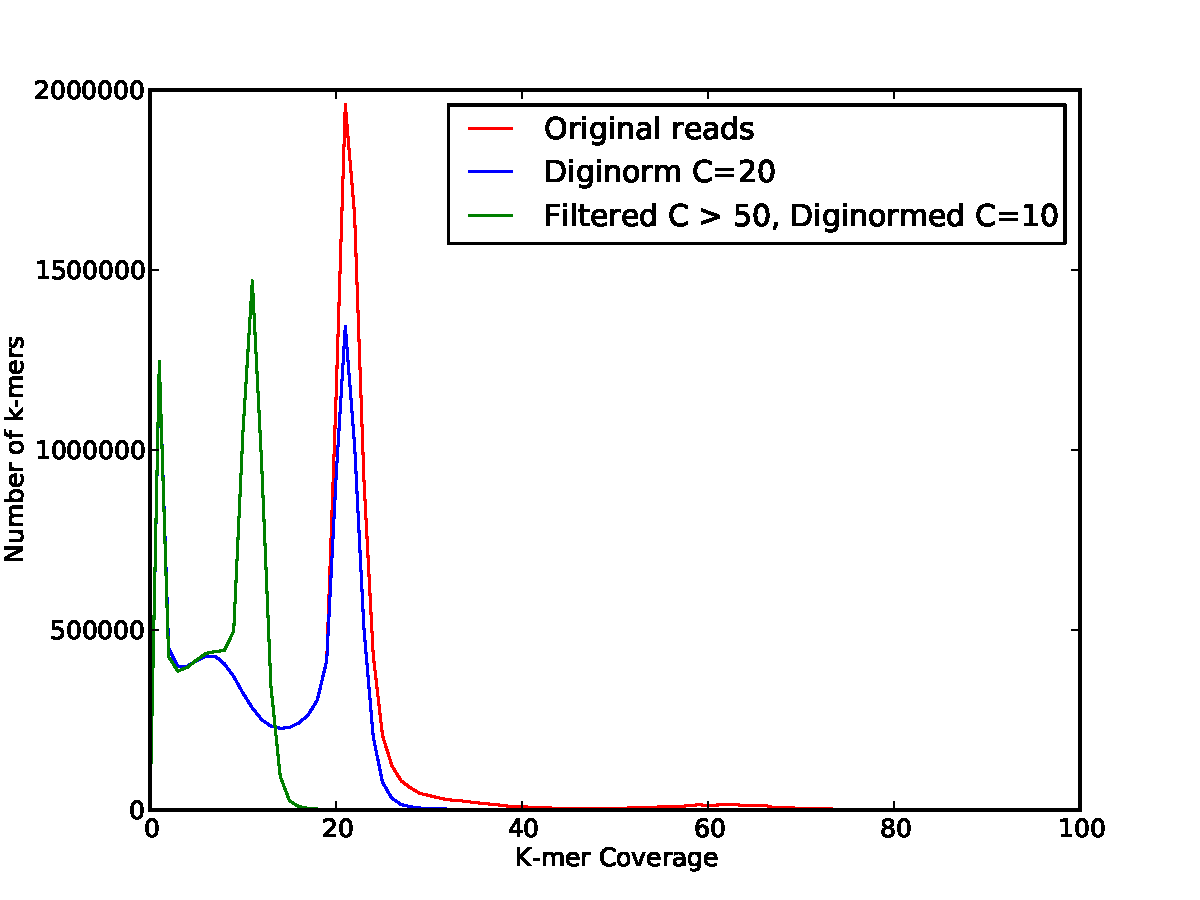
\includegraphics[width=\textwidth,height=\textheight,keepaspectratio]
{./figures/mockdiginormhist.pdf}}
\caption{  K-mer coverage of HMP mock community dataset before and after filtering approaches.}
\label{kmercoverage}
\end{figure}

\begin{figure}[ht]
\center{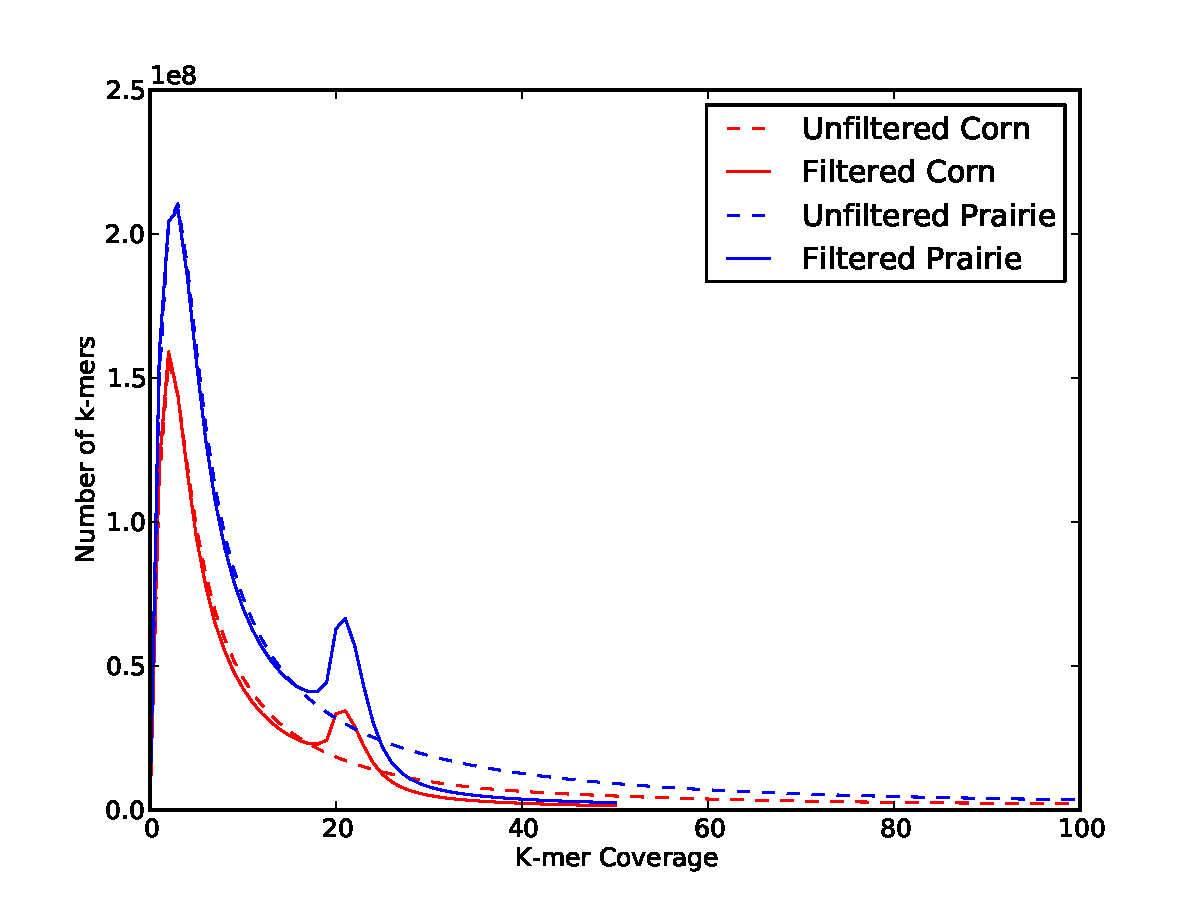
\includegraphics[width=\textwidth,height=\textheight,keepaspectratio]
{./figures/soildiginorm.pdf}}
\caption{K-mer coverage of Iowa corn and prairie metagenomes before and after filtering approaches.}
\label{diginormcoverage}
\end{figure}

\begin{figure}[ht]
\center{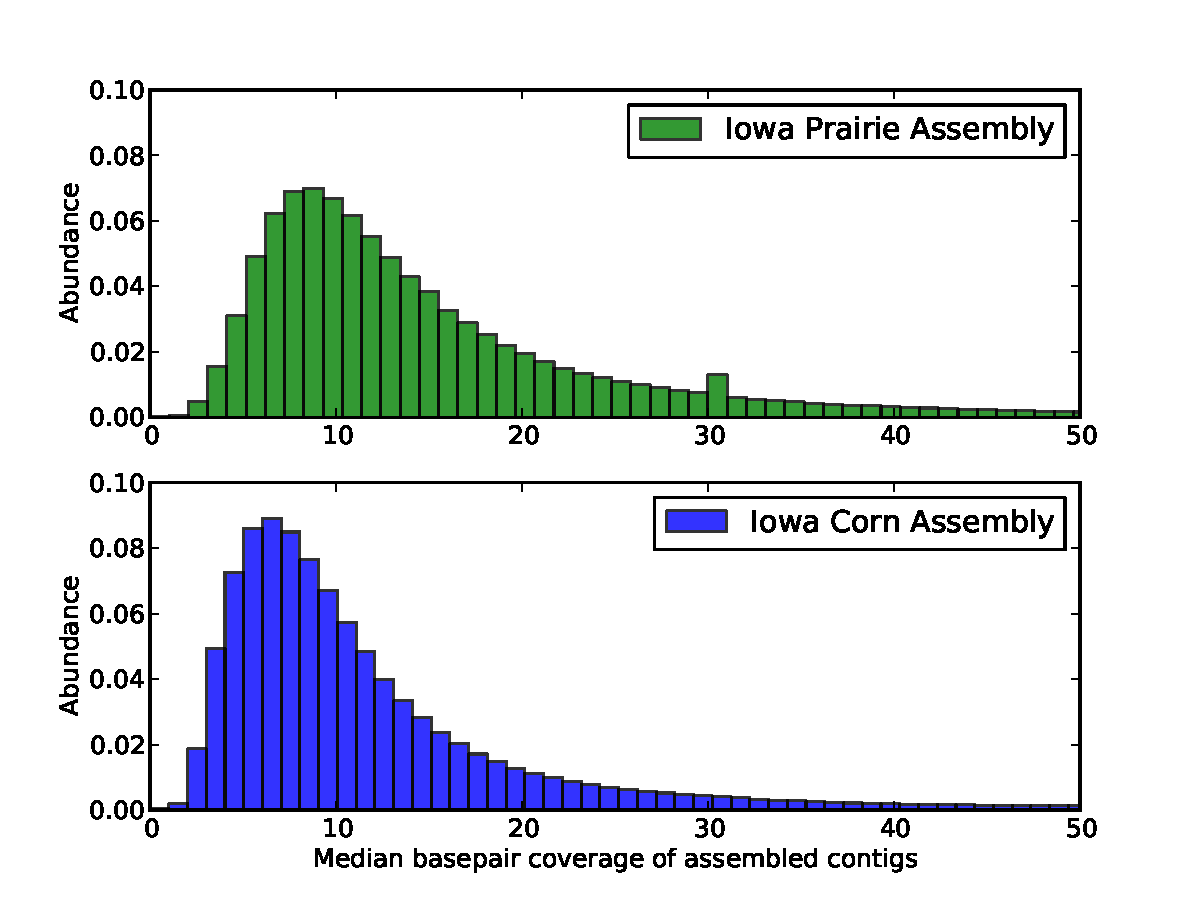
\includegraphics[width=\textwidth,height=\textheight,keepaspectratio]
{./figures/assembly-coverage.pdf}}
\caption{Coverage (median basepair) distribution of assembled contigs from soil metagenomes.}
\label{soilassemblycoverage}
\end{figure}

\begin{figure}[ht]
\center{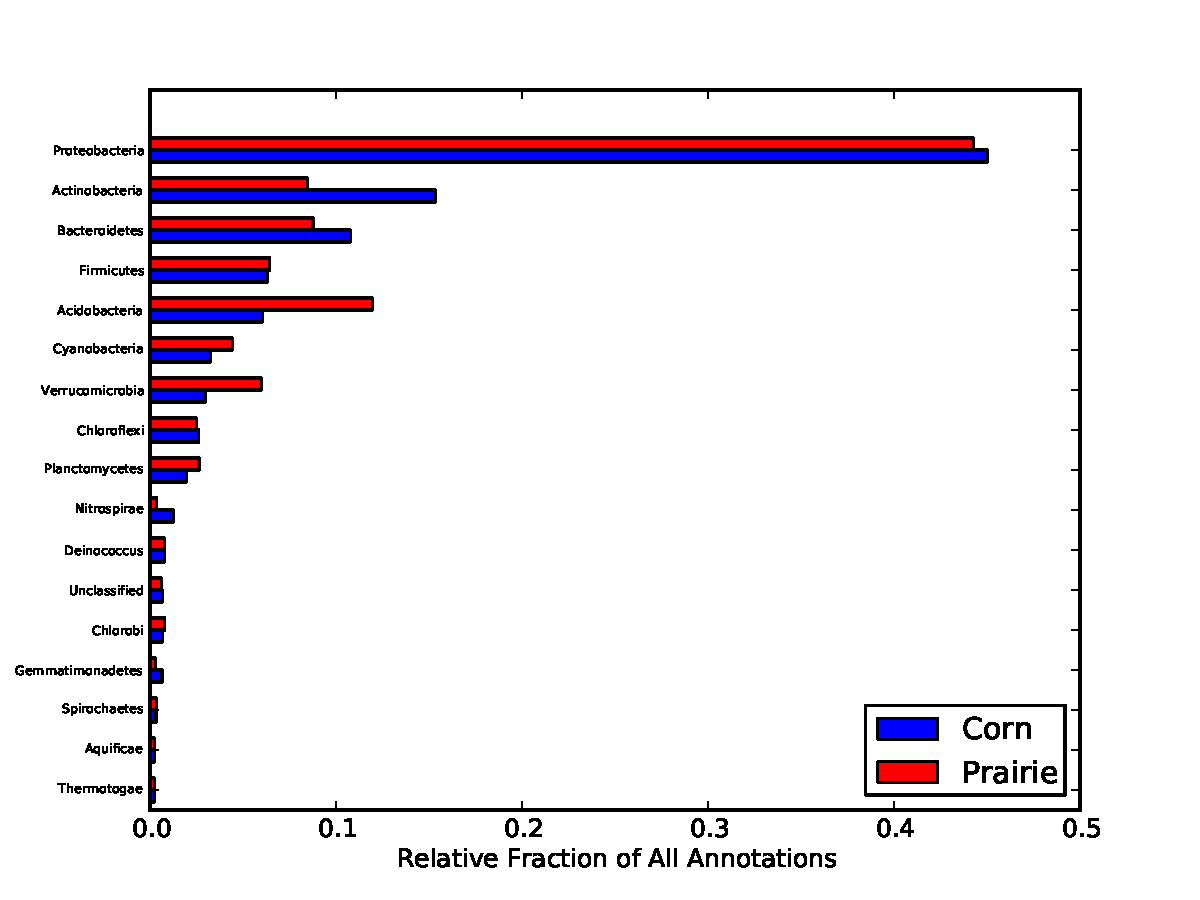
\includegraphics[width=\textwidth,height=\textheight,keepaspectratio]
{./figures/phyla.pdf}}
\caption{Phylogenetic distribution from SEED subsystem annotations for Iowa corn and prairie metagenomes.}
\label{phyla}
\end{figure}

\begin{figure}[ht]
\center{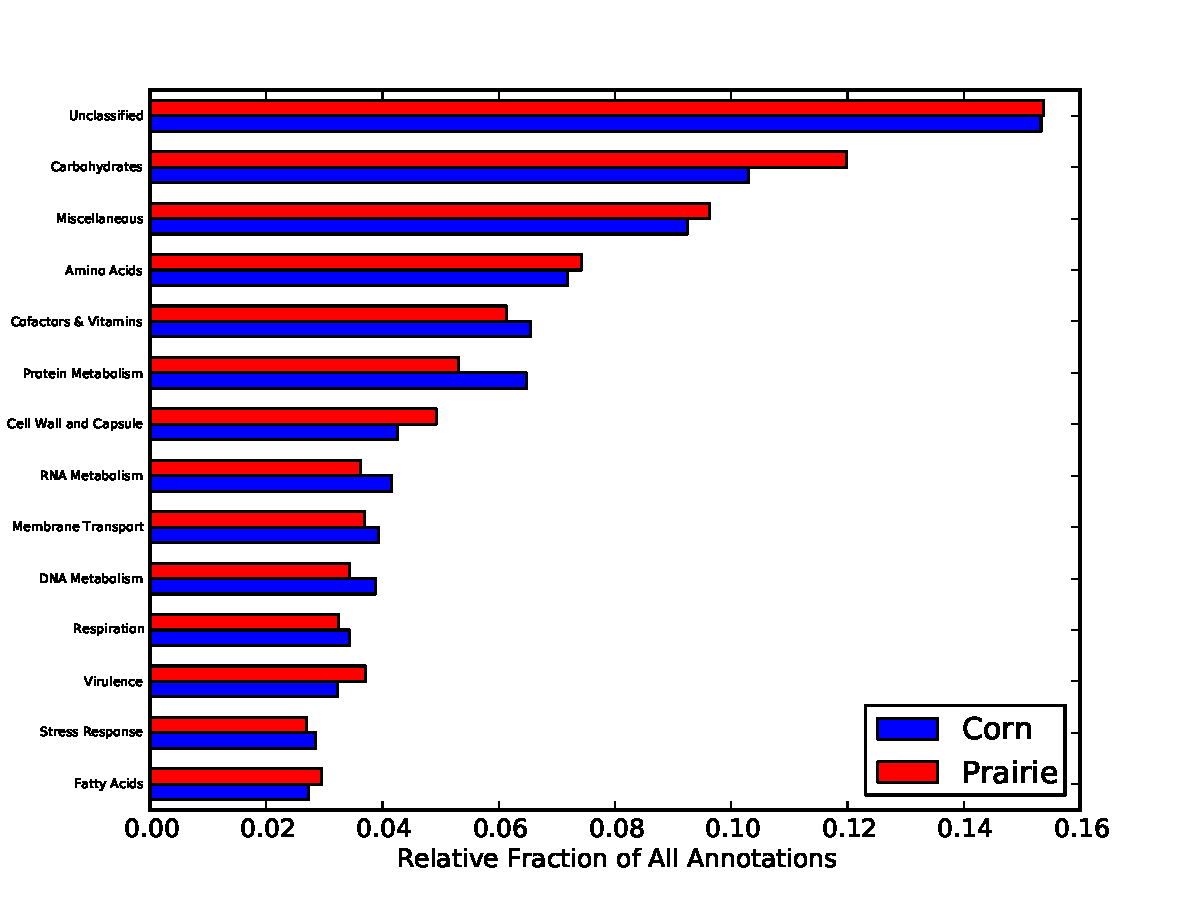
\includegraphics[width=\textwidth,height=\textheight,keepaspectratio]
{./figures/subsystems.pdf}}
\caption{Functional distribution from SEED subsystem annotations for Iowa corn and prairie metagenomes.}
\label{subsystem}
\end{figure}

\end{document}
